\documentclass[11pt]{ctexart}

\usepackage[a4paper,margin=22mm]{geometry}
\usepackage{amsmath,amssymb,booktabs,array,enumitem}
\usepackage{xcolor}
\usepackage{tikz}
\usepackage[colorlinks=true,linkcolor=blue,urlcolor=blue]{hyperref}

\usetikzlibrary{arrows.meta,positioning,fit,calc,shapes.geometric}

\definecolor{boxbg}{RGB}{242,239,255}
\definecolor{boxline}{RGB}{128,105,210}
\definecolor{warnbg}{RGB}{255,248,232}
\definecolor{warnline}{RGB}{190,140,40}
\definecolor{goodbg}{RGB}{236,248,241}
\definecolor{goodline}{RGB}{70,150,100}
\newcommand{\mask}{\texttt{[MASK]}}

\tikzset{
  box/.style={
    draw=boxline,
    fill=boxbg,
    rounded corners=2pt,
    align=center,
    inner sep=5pt,
    minimum height=8mm
  },
  smallbox/.style={
    draw=boxline,
    fill=boxbg,
    rounded corners=2pt,
    align=center,
    inner sep=4pt,
    font=\small
  },
  warnbox/.style={
    draw=warnline,
    fill=warnbg,
    rounded corners=2pt,
    align=center,
    inner sep=5pt
  },
  goodbox/.style={
    draw=goodline,
    fill=goodbg,
    rounded corners=2pt,
    align=center,
    inner sep=5pt
  },
  arrow/.style={-{Latex[length=2.3mm]}, thick},
  dashedarrow/.style={-{Latex[length=2.3mm]}, thick, dashed}
}

\title{Diffusion Language Models: 共同基础与优化问题入口}
\author{llmwiki / research-dlm}
\date{2026-07-16}

\begin{document}
\maketitle

\begin{abstract}
这份短稿的目的不是提出新算法，而是建立和数学、运筹、优化同学讨论 DLM 推理算法时的共同底座。
先把 ``diffusion process'' 分成连续扩散、一般离散扩散和 masked diffusion language model 三类；
再固定 masked DLM 的 forward/reverse 流程、状态、动作、约束和 baseline。
只有在这个基础上，新的优化算法才有清楚的对象、成本口径和 novelty 检验方式。
\end{abstract}

\section{先看哪个材料}

如果只看一份材料，先看本 PDF。它承担共同白板的角色。
然后按目的继续读：

\begin{center}
\begin{tabular}{p{0.25\linewidth}p{0.35\linewidth}p{0.28\linewidth}}
\toprule
目的 & 该看什么 & 不要先看什么 \\
\midrule
建立共同语言 & 本 PDF；\texttt{diffusion-process-visual.md} & 直接读 2026 sampler 论文 \\
讨论优化形式 & \texttt{math-or-discussion.md}；\texttt{optimization-bridge.md} & 泛泛说 ``用 DP/OR 会更好'' \\
检查想法新不新 & \texttt{paper/legacy/ideas/index.md}；\texttt{paper/legacy/ideas/audits/} & 只看自己算法的局部改进 \\
准备汇报 & \texttt{presentation-outline.md} & 堆论文列表 \\
\bottomrule
\end{tabular}
\end{center}

\section{三种不同的 ``解 diffusion''}

\begin{figure}[h]
\centering
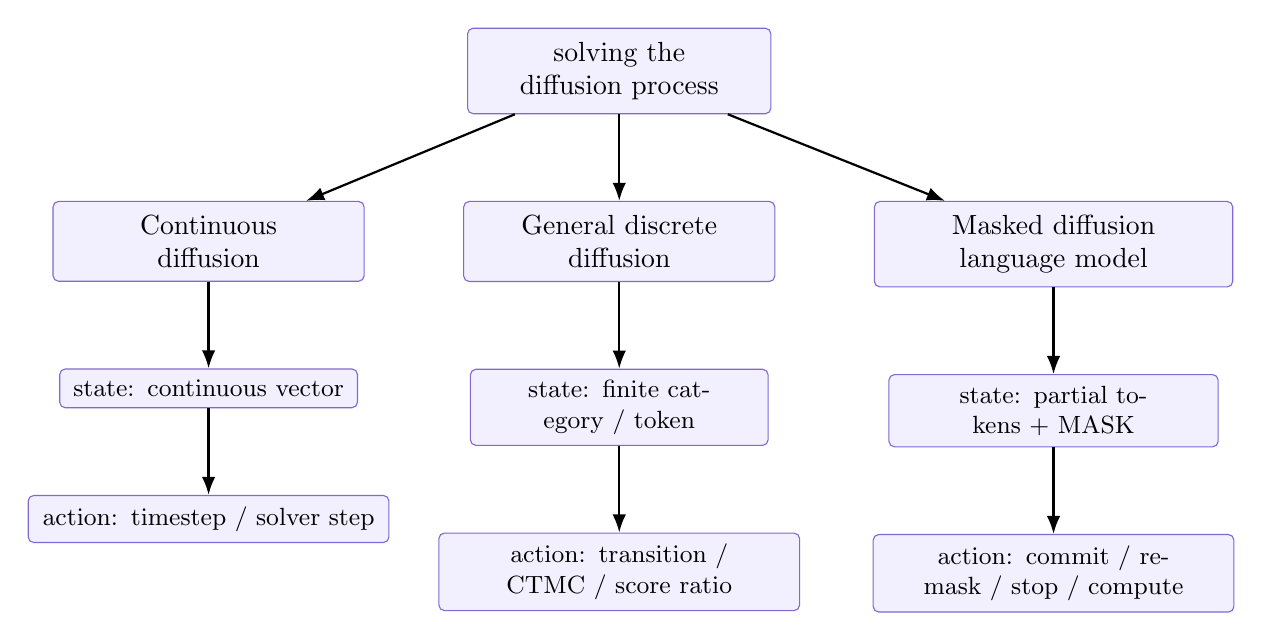
\begin{tikzpicture}[node distance=11mm and 13mm]
  \node[box, text width=35mm] (q) {solving the\\diffusion process};

  \node[box, text width=36mm, below left=of q] (cont) {Continuous\\diffusion};
  \node[box, text width=36mm, below=of q] (disc) {General discrete\\diffusion};
  \node[box, text width=42mm, below right=of q] (mdl) {Masked diffusion\\language model};

  \node[smallbox, text width=35mm, below=of cont] (conts) {state: continuous vector};
  \node[smallbox, text width=43mm, below=of conts] (conta) {action: timestep / solver step};

  \node[smallbox, text width=35mm, below=of disc] (discs) {state: finite category / token};
  \node[smallbox, text width=43mm, below=of discs] (disca) {action: transition / CTMC / score ratio};

  \node[smallbox, text width=39mm, below=of mdl] (mdls) {state: partial tokens + MASK};
  \node[smallbox, text width=43mm, below=of mdls] (mdla) {action: commit / remask / stop / compute};

  \draw[arrow] (q) -- (cont);
  \draw[arrow] (q) -- (disc);
  \draw[arrow] (q) -- (mdl);
  \draw[arrow] (cont) -- (conts);
  \draw[arrow] (conts) -- (conta);
  \draw[arrow] (disc) -- (discs);
  \draw[arrow] (discs) -- (disca);
  \draw[arrow] (mdl) -- (mdls);
  \draw[arrow] (mdls) -- (mdla);
\end{tikzpicture}
\caption{同一句 ``better algorithm for diffusion'' 可能指三个不同问题。本文后面主要讨论 masked DLM。}
\end{figure}

连续图像扩散常把问题写成 SDE/ODE 数值积分，核心是 time grid、local error、solver order。
masked DLM 的推理问题更像离散的 sequential subset control：每次模型 forward 后，要决定哪些位置提交、哪些位置撤销、是否额外计算，以及何时停止。
两者可以互相借思想，但不能把 ODE solver 的改名当成 DLM 解码算法。

\section{Masked DLM 的基础流程}

训练时的 forward process 把干净文本逐渐替换成 mask；生成时的 reverse process 从全 mask 或部分 mask canvas 恢复文本。

\begin{figure}[h]
\centering
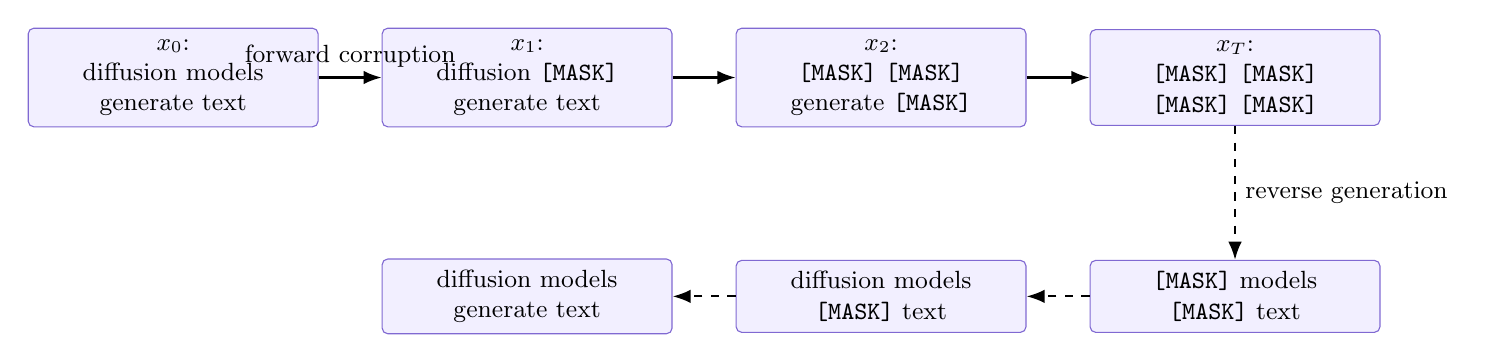
\begin{tikzpicture}[node distance=8mm]
  \node[smallbox, text width=34mm] (x0) {$x_0$:\\ diffusion models\\ generate text};
  \node[smallbox, text width=34mm, right=of x0] (x1) {$x_1$:\\ diffusion \mask\\ generate text};
  \node[smallbox, text width=34mm, right=of x1] (x2) {$x_2$:\\ \mask{} \mask\\ generate \mask};
  \node[smallbox, text width=34mm, right=of x2] (xt) {$x_T$:\\ \mask{} \mask\\ \mask{} \mask};

  \node[smallbox, text width=34mm, below=17mm of xt] (y2) {\mask{} models\\ \mask{} text};
  \node[smallbox, text width=34mm, left=of y2] (y1) {diffusion models\\ \mask{} text};
  \node[smallbox, text width=34mm, left=of y1] (y0) {diffusion models\\ generate text};

  \draw[arrow] (x0) -- node[above,font=\small] {forward corruption} (x1);
  \draw[arrow] (x1) -- (x2);
  \draw[arrow] (x2) -- (xt);
  \draw[dashedarrow] (xt) -- node[right,font=\small] {reverse generation} (y2);
  \draw[dashedarrow] (y2) -- (y1);
  \draw[dashedarrow] (y1) -- (y0);
\end{tikzpicture}
\caption{Absorbing-mask 直觉：token 随噪声时间进入 MASK；生成时模型逐步恢复 token。}
\end{figure}

单步反演可以抽象成下面的控制环。

\begin{figure}[h]
\centering
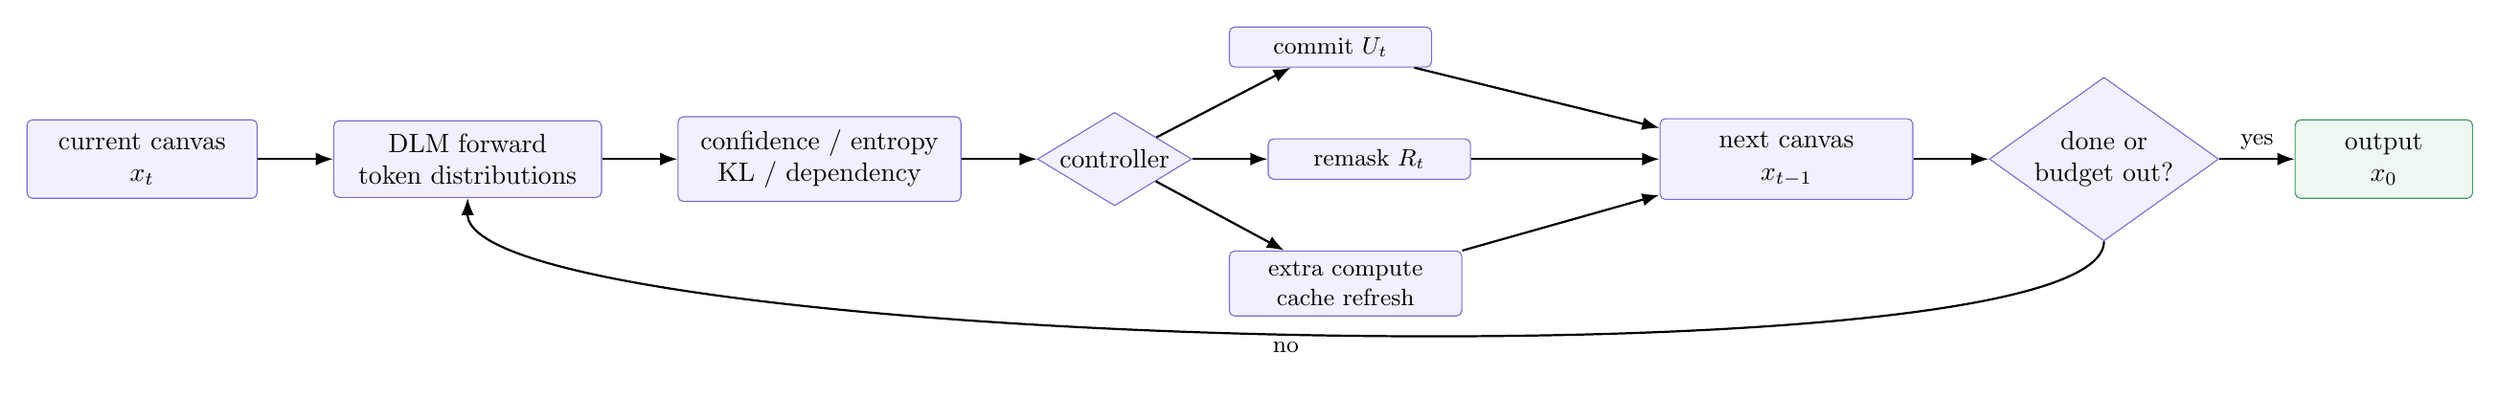
\begin{tikzpicture}[node distance=9mm and 10mm]
  \node[box, text width=27mm] (state) {current canvas\\$x_t$};
  \node[box, text width=32mm, right=of state] (forward) {DLM forward\\token distributions};
  \node[box, text width=34mm, right=of forward] (score) {confidence / entropy\\KL / dependency};
  \node[diamond, draw=boxline, fill=boxbg, aspect=1.65, align=center, right=of score, inner sep=1pt] (ctrl) {controller};

  \node[smallbox, text width=24mm, above right=of ctrl] (commit) {commit $U_t$};
  \node[smallbox, text width=24mm, right=of ctrl] (remask) {remask $R_t$};
  \node[smallbox, text width=28mm, below right=of ctrl] (extra) {extra compute\\cache refresh};
  \node[box, text width=30mm, right=25mm of remask] (next) {next canvas\\$x_{t-1}$};
  \node[diamond, draw=boxline, fill=boxbg, aspect=1.4, align=center, right=of next, inner sep=1pt] (done) {done or\\budget out?};
  \node[goodbox, text width=20mm, right=of done] (out) {output\\$x_0$};

  \draw[arrow] (state) -- (forward);
  \draw[arrow] (forward) -- (score);
  \draw[arrow] (score) -- (ctrl);
  \draw[arrow] (ctrl) -- (commit);
  \draw[arrow] (ctrl) -- (remask);
  \draw[arrow] (ctrl) -- (extra);
  \draw[arrow] (commit) -- (next);
  \draw[arrow] (remask) -- (next);
  \draw[arrow] (extra) -- (next);
  \draw[arrow] (next) -- (done);
  \draw[arrow] (done) -- node[above,font=\small] {yes} (out);
  \draw[arrow] (done.south) .. controls +(0,-20mm) and +(0,-20mm) .. node[below,font=\small] {no} (forward.south);
\end{tikzpicture}
\caption{Masked DLM sampler 本质上在控制每次 forward 之后的离散动作。}
\end{figure}

\section{优化开发时要固定的数学接口}

最小状态和动作可以写成
\[
s_t=(x_t, M_t, \ell_t, h_t, c_t, b_t),
\]
其中 $x_t$ 是当前 canvas，$M_t$ 是 mask 集合，$\ell_t$ 是 logits 或派生 score，$h_t$ 是历史轨迹，$c_t$ 是 cache 或系统状态，$b_t$ 是剩余预算。
动作可以写成
\[
a_t=(U_t, R_t, m_t, \mathrm{stop}),
\]
其中 $U_t$ 是要 commit 的位置集合，$R_t$ 是要 remask 或验证的位置集合，$m_t$ 是计算模式。

在固定模型调用预算 $B$ 下，一个基础问题是
\[
\max_{\pi}\; \mathbb{E}[Q(x_0)]
\quad
\text{s.t.}\quad
\sum_t \mathrm{NFE}_t \le B,\qquad M_0=\varnothing.
\]

在服务系统里，更合理的约束可能是
\[
\min_{\pi}\; \mathrm{p95\_latency}
\quad
\text{s.t.}\quad
\mathbb{P}(\mathrm{task\ failure})\le \alpha,\qquad
\mathrm{memory}\le C.
\]

因此，新的优化算法必须同时说明四件事：
\begin{enumerate}[leftmargin=18pt]
  \item 它访问什么信息：confidence、entropy、attention、trajectory、cache drift、额外模型，还是 ground truth。
  \item 它优化什么成本：NFE、wall-clock、p50/p95、显存、batch interaction，还是 controller overhead。
  \item 它改变哪个动作：更新多少、更新哪些、是否撤销、是否搜索、是否刷新 cache。
  \item 它怎样被杀掉：哪个 matched-cost 实验会证明这个机制没有用。
\end{enumerate}

\section{为什么简单 top-k 不够}

并行预测会给每个位置一个局部分布，但语言输出的正确性是序列级的。
两个位置各自高 confidence，并不保证它们同时提交后兼容。

\begin{figure}[h]
\centering
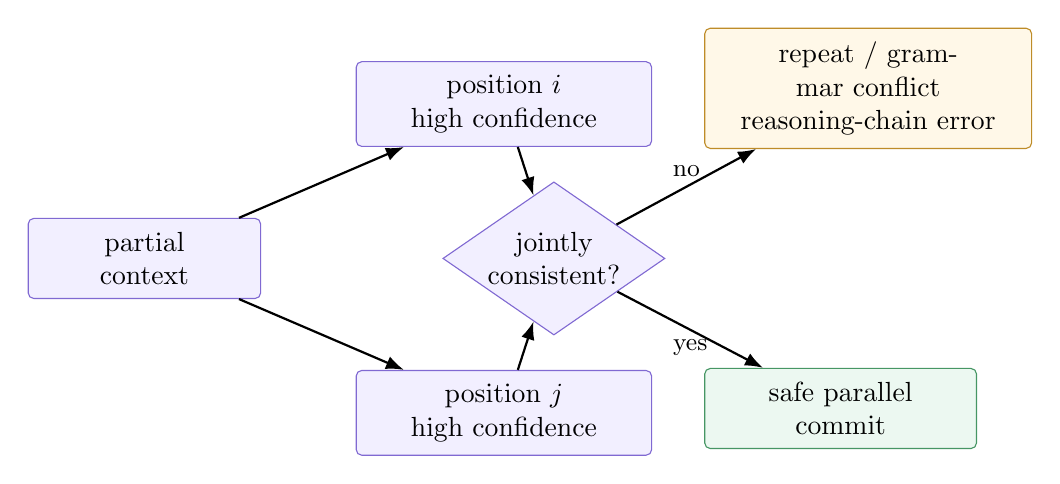
\begin{tikzpicture}[node distance=9mm and 12mm]
  \node[box, text width=26mm] (ctx) {partial\\context};
  \node[box, text width=34mm, above right=of ctx] (i) {position $i$\\high confidence};
  \node[box, text width=34mm, below right=of ctx] (j) {position $j$\\high confidence};
  \node[diamond, draw=boxline, fill=boxbg, aspect=1.45, align=center, right=23mm of ctx, inner sep=1pt] (joint) {jointly\\consistent?};
  \node[warnbox, text width=38mm, above right=of joint] (bad) {repeat / grammar conflict\\reasoning-chain error};
  \node[goodbox, text width=31mm, below right=of joint] (good) {safe parallel\\commit};

  \draw[arrow] (ctx) -- (i);
  \draw[arrow] (ctx) -- (j);
  \draw[arrow] (i) -- (joint);
  \draw[arrow] (j) -- (joint);
  \draw[arrow] (joint) -- node[above,font=\small] {no} (bad);
  \draw[arrow] (joint) -- node[below,font=\small] {yes} (good);
\end{tikzpicture}
\caption{DLM 优化的难点之一：局部置信度不是序列正确性的充分统计量。}
\end{figure}

这也是为什么现有工作会研究 dependency-aware subset selection、rollback/remasking、lookahead、learned policy 和 cache correctness。
一个新算法如果只把 score 从 confidence 换成另一个局部启发式，通常不够。

\section{新算法放进来时的检查表}

\begin{center}
\begin{tabular}{p{0.24\linewidth}p{0.32\linewidth}p{0.34\linewidth}}
\toprule
算法类型 & 最近邻 baseline & 最低检验 \\
\midrule
更新多少 token & EB-Sampler, Fast-dLLM, progress schedules & matched NFE 与真实 wall-clock \\
更新哪些 token & DUS, ADAS, CLAD, AXON & confidence-matched 负对照 \\
撤销/验证 token & Saber, WINO, RACC, NAVIRA & 修复收益是否超过 overhead \\
搜索多条轨迹 & MEDAL, LookUM & 额外 forward 是否公平计入 \\
cache / systems & dKV, Elastic-Cache, SPA, COVER, dInfer & p50/p95、显存、cache correctness \\
\bottomrule
\end{tabular}
\end{center}

和同学讨论时，最后应留下五行，而不是留下一个模糊口号：
\[
\begin{array}{ll}
\textbf{Problem:} & \text{具体解哪个 DLM 推理失败模式？}\\
\textbf{Closest prior:} & \text{最像哪篇工作？}\\
\textbf{Delta:} & \text{唯一不同的机制是什么？}\\
\textbf{Budget:} & \text{NFE、wall-clock、p95、显存怎样计？}\\
\textbf{Kill test:} & \text{哪个小实验会杀掉这个 claim？}
\end{array}
\]

\section{建议的下一步}

先不要直接写新算法。更稳的顺序是：
\begin{enumerate}[leftmargin=18pt]
  \item 复现两个强 sampler，在同一 open DLM 上得到 quality--latency frontier。
  \item 做 controlled shift：换任务、长度、模型或输出分布，观察 controller 是否失准。
  \item 如果失准，定义可观测的 residual failure；如果没有失准，说明算法空间可能已经被现有方法覆盖。
  \item 让新算法只针对这个 residual failure 提出机制，并用 matched-cost negative control 检验。
\end{enumerate}

\end{document}
